\documentclass[a4paper,12pt]{article} 

\usepackage[top = 2.5cm, bottom = 2.5cm, left = 2.5cm, right = 2.5cm]{geometry} 

% packages
\usepackage{amsmath, amsfonts, amsthm} % basic math packages
\usepackage{tikz} % for making illustrations
\usetikzlibrary{shapes.arrows, arrows, decorations.markings, positioning}
\usetikzlibrary{calc}
\usetikzlibrary{3d}
\usepackage{graphicx} % for importing images
\usepackage{xcolor} % more color options
\usepackage{colortbl}
\usepackage{multicol} % for making two-column lists
\usepackage{hyperref} % for hyperlinking
%\hypersetup{colorlinks=true, urlcolor=cyan,}
\usepackage{mathabx}
\usepackage{cleveref}
\usepackage{subfig}
\usepackage{array}
\usepackage{wrapfig}
\usepackage{bbm}
\usepackage{fancyhdr}
\usepackage{algorithm, algorithmicx, algpseudocode}
\usepackage{stmaryrd}
\usepackage{physics}
\usepackage{mwe}


% The following two packages - multirow and booktabs - are needed to create nice looking tables.
\usepackage{multirow} % Multirow is for tables with multiple rows within one cell.
\usepackage{booktabs} % For even nicer tables.

% As we usually want to include some plots (.pdf files) we need a package for that.
\usepackage{graphicx} 

% The default setting of LaTeX is to indent new paragraphs. This is useful for articles. But not really nice for homework problem sets. The following command sets the indent to 0.
\usepackage{setspace}
\setlength{\parindent}{0in}

% Package to place figures where you want them.
\usepackage{float}

% The fancyhdr package let's us create nice headers.
\usepackage{fancyhdr}

% theorems, lemmas, examples, etc.
\newtheorem{theorem}{Theorem}[section]
% \newtheorem{corollary}{Corollary}[theorem]
% \newtheorem{lemma}[theorem]{Lemma}
\newtheorem{example}[theorem]{Example}
\newtheorem{lemma}[theorem]{Lemma}
\theoremstyle{definition}
\newtheorem{definition}{Definition}[section]
\theoremstyle{remark}
\newtheorem*{remark}{Remark}
\newtheorem*{solution}{Solution}

\def\mydefb#1{\expandafter\def\csname bf#1\endcsname{\mathbf{#1}}}
\def\mydefallb#1{\ifx#1\mydefallb\else\mydefb#1\expandafter\mydefallb\fi}
\mydefallb aAbBcCdDeEfFgGhHiIjJkKlLmMnNoOpPqQrRsStTuUvVwWxXyYzZ\mydefallb

\def\mydefb#1{\expandafter\def\csname cal#1\endcsname{\mathcal{#1}}}
\def\mydefallb#1{\ifx#1\mydefallb\else\mydefb#1\expandafter\mydefallb\fi}
\mydefallb aAbBcCdDeEfFgGhHiIjJkKlLmMnNoOpPqQrRsStTuUvVwWxXyYzZ\mydefallb

\def\mydefgreek#1{\expandafter\def\csname bf#1\endcsname{\text{\boldmath$\mathbf{\csname #1\endcsname}$}}}
\def\mydefallgreek#1{\ifx\mydefallgreek#1\else\mydefgreek{#1}%
	\lowercase{\mydefgreek{#1}}\expandafter\mydefallgreek\fi}
\mydefallgreek {alpha}{Alpha}{beta}{Beta}{gamma}{Gamma}{delta}{Delta}{epsilon}{Epsilon}{varepsilon}{Varepsilon}{zeta}{Zeta}{eta}{Eta}{theta}{Theta}{iota}{Iota}{kappa}{Kappa}{lambda}{Lambda}{mu}{Mu}{nu}{Nu}{omicron}{Omicron}{pi}{Pi}{rho}{Rho}{sigma}{Sigma}{tau}{Tau}{upsilon}{Upsilon}{varphi}{phi}{Phi}{xi}{Xi}{chi}{Chi}{psi}{Psi}{omega}{Omega}\mydefallgreek

%% Change this to just the normal N,Z,R,C,P,E
\def\mydefb#1{\expandafter\def\csname bb#1\endcsname{\mathbb{#1}}}
\def\mydefallb#1{\ifx#1\mydefallb\else\mydefb#1\expandafter\mydefallb\fi}
\mydefallb CEGIKNPQRST\mydefallb

\newcommand{\half}{\frac{1}{2}}
\DeclareMathOperator{\sgn}{sgn}
\DeclareMathOperator*{\argmax}{arg\,max}
\DeclareMathOperator*{\argmin}{arg\,min}
\DeclareMathOperator{\prox}{prox}
\newcommand{\matlab}{\textsc{Matlab}}


%%%%%%%%%%%%%%%%%%%%%%%%%%%%%%%%%%%%%%%%%%%%%%%%
% 3. Header (and Footer)
%%%%%%%%%%%%%%%%%%%%%%%%%%%%%%%%%%%%%%%%%%%%%%%%

% To make our document nice we want a header and number the pages in the footer.

\pagestyle{fancy} % With this command we can customize the header style.

\fancyhf{} % This makes sure we do not have other information in our header or footer.

\lhead{\footnotesize CS 534:  Homework  \# 3}% \lhead puts text in the top left corner. \footnotesize sets our font to a smaller size.

%\rhead works just like \lhead (you can also use \chead)
\rhead{\footnotesize Scott (mtscot4)} %<---- Fill in your lastnames.

% Similar commands work for the footer (\lfoot, \cfoot and \rfoot).
% We want to put our page number in the center.
\cfoot{\footnotesize \thepage} 

\begin{document}
	
	
	%%%%%%%%%%%%%%%%%%%%%%%%%%%%%%%%%%%%%%%%%%%%%%%%
	%%%%%%%%%%%%%%%%%%%%%%%%%%%%%%%%%%%%%%%%%%%%%%%%
	
	%%%%%%%%%%%%%%%%%%%%%%%%%%%%%%%%%%%%%%%%%%%%%%%%
	% Title section of the document
	%%%%%%%%%%%%%%%%%%%%%%%%%%%%%%%%%%%%%%%%%%%%%%%%
	
	% For the title section we want to reproduce the title section of the Problem Set and add your names.
	
	\thispagestyle{empty} % This command disables the header on the first page. 
	
	\begin{tabular}{p{15.5cm}} % This is a simple tabular environment to align your text nicely 
		{\large \sc CS 534:  Machine Learning} \\
		Emory University \\ Fall2024 \\ Prof. Eugene Agichtein \\
		\hline % \hline produces horizontal lines.
		\\
	\end{tabular} % Our tabular environment ends here.
	
	\vspace*{0.3cm} % Now we want to add some vertical space in between the line and our title.
	
	\begin{center} % Everything within the center environment is centered.
		{\Large \bf Homework \# 3} % <---- Don't forget to put in the right number
		\vspace{2mm}
		
		% YOUR NAMES GO HERE
		{\bf Mitchell Scott}\\ (mtscot4) % <---- Fill in your names here!
		
	\end{center}  
	
	\vspace{0.4cm}
	
	%%%%%%%%%%%%%%%%%%%%%%%%%%%%%%%%%%%%%%%%%%%%%%%%
	%%%%%%%%%%%%%%%%%%%%%%%%%%%%%%%%%%%%%%%%%%%%%%%%
	
	% Up until this point you only have to make minor changes for every week (Number of the homework). Your write up essentially starts here.
	
	\begin{enumerate}
		\item {\bf Energy appliance regression} (50 pts, written + code):\\
		We again use the Energy dataset ({\tt energydata.zip}) from Homework \#1. As a reminder, each sample contains
		measurements of temperature and humidity sensors from a wireless network, weather from a nearby airport station,
		and the recorded energy use of lighting fixtures to predict the energy consumption of appliances in a low energy
		house. Put all code into \texttt{q1.py}. There are 2 classes: \texttt{FeatureSelection} and \texttt{Regression}. Complete implementation of the following class methods. You may use helper methods from the {\tt sklearn.feature\_selection} module and regressors from {\tt sklearn.linear\_model}.
		\begin{enumerate}
			\item {\bf Code:} {\tt FeatureSelection.rank\_correlation(x, y)} that takes in a numpy 2d array, $\bfx$, a numpy 1d array, $\bfy$, and returns the rank of the features in $\bfx$ based on Pearson correlation of each individual feature to the target value. The function should return a numpy array in descending order of the most correlated feature column (i.e., [3, 1,
			0, 2] would mean that the 4th feature has the highest correlation to $\bfy$ followed by 2nd, then 1st , and lastly 3rd
			feature.)
			\begin{solution}
				Implimented in \texttt{q1.py}.
			\end{solution}
			\item {\bf Code:} {\tt FeatureSelection.Lasso(x, y) } that takes in a numpy 2d array, $\bfx$, a numpy 1d array, $\bfy$, and returns the rank of the features in $\bfx$ based on coefficients of Lasso regression ($\ell^1$ regularization). The function should return a numpy array in descending order of the absolute magnitude of Lasso regression coefficient. do not
			include features with zero Lasso coefficient. For example, for 4-features input $\bfX$, if Lasso coefficients are [2.3,
			-4.5, 0, 7.6], we should return [3, 1, 0], to mean that the 4th feature has the highest coefficient followed by 2nd, then 1st , , and the 3rd feature is dropped. Note that the returned array is likely to be shorter than the original
			dimension of $\bfX$.
			\begin{solution}
				Implimented in \texttt{q1.py}.
			\end{solution}
			\item {\bf Code:} {\tt FeatureSelection.stepwise(x, y)} that takes in a numpy 2d array, $\bfx$, a numpy 1d array, $\bfy$, and returns the rank of the features in $\bfx$ based by greedy adding one remaining feature at a time to the set. To do this, we try adding one remaining feature at a time to the set, train a linear regressor, and select next feature to add based on the highest decrease in RMSE. Stop the process when RMSE does not decrease. For simplicity, we do this process on the training set $\bfX$, but feel free to use cross validation for this step. See slides for details or read about reference implementation SequentialFeatureSelector. Return ranking of features in descending order of importance. Note that the returned array is likely to be shorter than the original dimension of $\bfX$.
			\begin{solution}
					Implimented in \texttt{q1.py}.
			\end{solution}
			\item {\bf Written:} report up to 10 first features selected by each method 1a,1b, and 1c in a table. Comment on overlap and
			differences in the resulting feature sets.
			\begin{solution}
				For the {\tt rank\_correlation} method, we arrived at $[24, 23,  8, 10,  9,\cdots$ $20,  6, 17, 22,  2]$. For the {\tt lasso} method, we arrived at, $[12, 22, 21, 20, 19, 17, 15,\cdots$ $ 14, 13, 24]$. Lastly, For the {\tt stepwise} method, we arrived at, $[12, 22, 20, 19, 17, \cdots$ $15, 14, 10, 24,  7]$. We see that {\tt lasso} and {\tt stepwise} give rather similar results with the first 7 out of 8 entries being the same. Additionally, we see 24 represented close to the bottom in both methods as well. Comparing either {\tt lasso} or {\tt stepwise} with {\tt rank\_correlation}, we see that the results are not all that similar. Of course all methods have 24, 20, 17, and 22, but whereas, {\tt lasso} starts with 22,20, and 17, {\tt rank\_correlation} has those entries at the end. Conversely, {\tt stepwise } has 24 as one of the last, but {\tt rank\_correlation} has it first. 
				
				Additionally, while {\tt lasso} and {\tt stepwise} have very similar results, {\tt stepwise} took noticibly longer to compute.
			\end{solution}
			\item {\bf Code:} {\tt Regression.Ridge(train\_x, train\_y, test\_x, test\_y):} Implement Ridge regression and returns prediction on test set similar to HW1. You may use {\tt sklearn} for the regressor implementation
			\begin{solution}
				 Implimented in \texttt{q1.py}.
			\end{solution}
			\item {\bf Written:} use your code in 1e to train and test Ridge regression on the whole feature set (“No selection”), and on
			top 10 features selected in 1a, 1b, 1c. Report in a table the RMSE and R$^2$ of the Ridge regressor on the
			validation dataset and test dataset. Comment on differences/similarities of performance of Ridge regression
			under the different feature selection methods.
			\begin{solution}
				As we can see in Tab \ref{tab:selectionmethods}, by training on the full data set, we get considerably better training and test RMSE and R$^2$.
			\begin{table}
				\centering
				\begin{tabular}{|c|c|c|c|c|}
					\hline
					Selection Method&Train RMSE  &Train r2  &Test RMSE  & Test r2  \\
					\hline\hline
					Full& {\bf 0.94963}& {\bf0.18675} & {\bf0.95906} & {\bf -0.21560}\\
					Correlation&	0.49582  & 0.71419 & 1.41650 & -8.79686 \\
					Lasso&  0.56684& 0.88240 &  0.97312& -1.49702 \\
					Stepwise&  0.78201& 0.59070 & 1.05242 & -2.13966 \\
					\hline
				\end{tabular}
				\caption{By changing the features selected, we see drastically different training and test accuracies.}
				\label{tab:selectionmethods}
			\end{table}
			\end{solution}
			\item {\bf Code:} {\tt Regression.DecisionTreeRegressor (train\_x, train\_y, test\_x, test\_y, max\_depth, min\_items):}
			Implement Regression Tree training and prediction, and return prediction on validation and test sets similar to
			HW1. You may use sklearn for the underlying regressor tree implementation.
			\begin{solution}
			Implimented in \texttt{q1.py}.
			\end{solution}
			\item {\bf Written:} tune the hyperpameters of your regression tree in 1g on whole feature set by varying the {\tt max\_depth}
			and {\tt min\_items} and selecting the best configuration based on the validation set. Report the best configuration
			and RMSE and R$^2$ obtained on validation set.
			\begin{solution}
				By iterating over \texttt{max\_depth = } [2,5,8], \texttt{min\_items} = [1,3,5], we were able to see the dependence on these parameters in terms of training the regression tree. (2,5) won. Alll results are seen in Tab \ref{tab:tuning_dtr_params}.
				\begin{table}
					\centering
					\begin{tabular}{|c|cc|cc|}
						\hline
						\begin{tabular}{c}
							Parameters\\
							({\tt max\_depth, min\_items})
						\end{tabular}& Train RMSE & Train r2 & Test RMSE & Test r2\\
						\hline\hline
						(2,1) & 0.97108 & 0.11075 & 0.92638 & -0.05817\\
						(2,3) & 0.97108 & 0.11075 & 0.92638 & -0.05817\\
						(2,5) & {\bf 0.97108 }& {\bf0.11075} & {\bf0.92638} & {\bf-0.05817}\\
						\hline
						(5,1) & 0.92628 & 0.26386 & 1.01166 & -0.50499\\
						(5,3) & 0.92536 & 0.26678 & 1.01166 & -0.50499\\
						(5,5) & 0.92620 & 0.26411  & 1.01166 & -0.50499\\
						\hline
						(8,1) & 0.83043 & 0.52443 & 1.07061 & -0.88766\\
						(8,3) & 0.83169 & 0.52155  & 1.02947 & -0.61385\\
						(8,5) & 0.84739 & 0.49882 & 1.02207 & -0.56794\\
						\hline
					\end{tabular}
					\caption{Tuning the hyperparameters for a Decision Tree Regressor. Bolded is best.}
					\label{tab:tuning_dtr_params}
				\end{table}
			
			
			\end{solution}
			\item {\bf Written:} Train the regressor using best configuration on full dataset as training (train’=train+validation), and report RMSE and R$^2$ on test dataset. Compare performance of your tree regressor to the best performance of Ridge regression in 1f.
			\begin{solution}
				Using the full data set, we computed, the following dictionary:
				\[\{\texttt{'test-rms'}: 0.90088, \quad \texttt{'test-r2'}: 0.05363.\}\]
				We are able to see that our test RMSE is lower and our R$^2$ value is more positive but smaller in magnitude. I feel that a positive correlation is better, so a success on both counts.
			\end{solution}
			\item {\bf Written:} visualize top 3 levels in your decision tree in 1h and 1i. Compare the top-level features used by your
			tree, with the features selected in 1d. Comment on overlap/order of importance of features in the two methods.
			\begin{solution}
				We see the decision trees for 1h and 1i in Fig \ref{fig:1h} and Fig. \ref{fig:1i}, respectively. 17 appears in both, which is good because feature 17 was mentioned in every single feature selection method.16 and 21 were mentioned once each and were mentioned in just one of the feature selection methods.
				\begin{figure}
				\centering
				\begin{minipage}{0.49\textwidth}
					\centering
					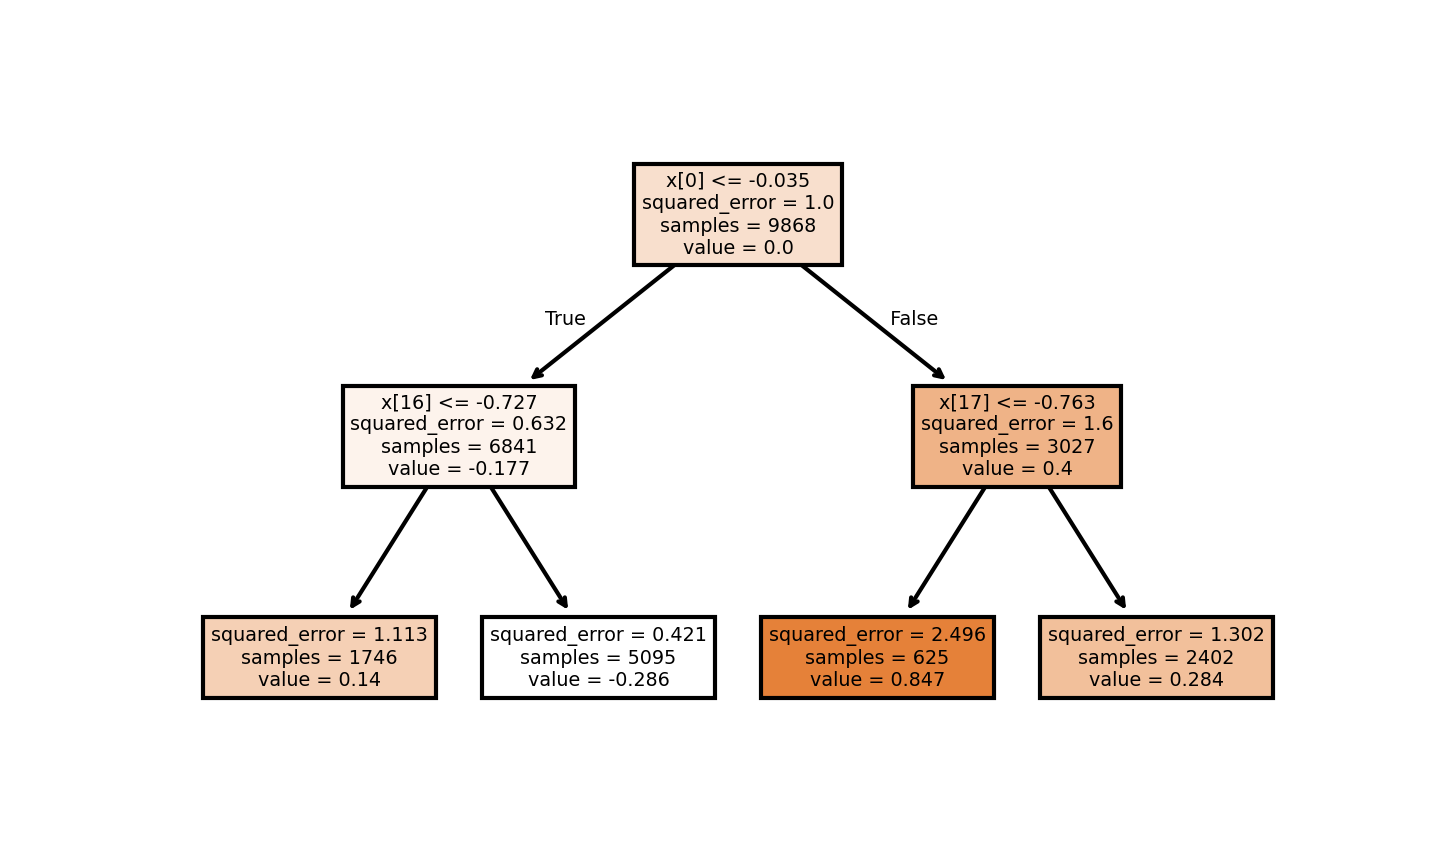
\includegraphics[width=0.95\textwidth]{../decision_tree_h}
					\caption{Decision Tree H}
					\label{fig:1h}
				\end{minipage}\hfill
				\begin{minipage}{0.49\textwidth}
					\centering
					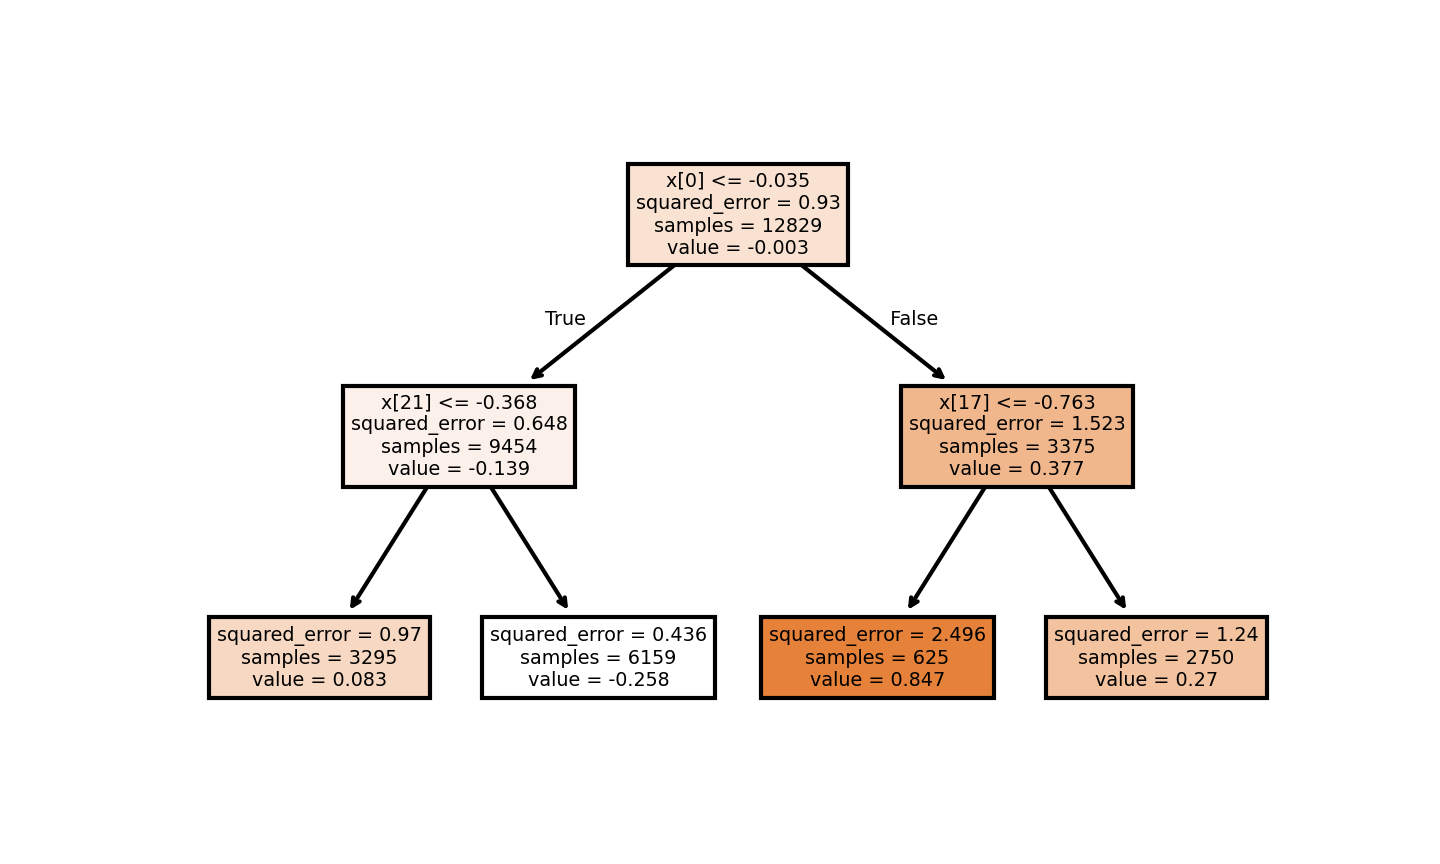
\includegraphics[width=0.95\textwidth]{../decision_tree_i} % second figure itself
					\caption{Decision Tree I}
					\label{fig:1i}
				\end{minipage}
				\end{figure}
			\end{solution}
		\end{enumerate}
		\item {\bf Spam classification using Naïve Bayes, Random Forest, and GBDT} (50  pts, written + code):
		We will use the same email spam dataset from HW2 the email spam dataset, which contains 4601 e-mail messages
		that have been split into 3000 training (spam.train.dat) and 1601 test emails (spam.test.dat). 57 features have been
		already extracted for you, with a binary label in the last column.
		All the specified functions should be in the file \texttt{‘q2.py’}.
		\begin{enumerate}
			\item {\bf Code:} Write a Python function {\tt eval\_randomforest(trainx, trainy, testx, testy, num\_trees, max\_depth, min\_items)} that fits a Random Forest model to the training data. You can use sklearn module for this part. The
			function should accept as input numpy 2d arrays, and return a dictionary containing the accuracy and AUC for the
			training and test sets and the predicted probabilities for the test set: {\tt return \{"train-acc": train\_acc, "train-auc":
				train\_auc, "test-acc": test\_acc, "test-auc": test\_auc, "test-prob": test\_prob\}}. The values for accuracy and AUC should be scalar numeric values, while test-prob should be a numpy 1-d array with the predicted probability for the positive class 1, for the test. Same format as HW2.
			\begin{solution}
				 Implimented in \texttt{q3.py}.
			\end{solution}
			\item  {\bf Written:} Tune RandomForest for the Spam classification problem by optimizing the hyperparameters
			{\tt num\_trees, max\_depth, min\_items} based on cross validation over the training set only. Report best configuration,
			and average AUC and Accuracy across validation folds.
			\begin{solution}
				By going from 1 to 16 estimators, 1 to 15 depth and 1 to 15 items per leaf, we found that the best was 16 estimators, max depth of 15 and 9 min items. The resulted in the following corss validated data.\\
				
				{'train-acc': 0.95043, 'train-auc': 0.94303, 'val-acc': 0.93263, 'val-auc': 0.92469}
			\end{solution}
			\item {\bf Written:} Train Random forest on all training data with using best hyperparameters identified in 2b, and report
			AUC, F1, and Accuracy on the test set. Compare in a table to the performance to NB and LR from Homework 2.
			\begin{solution}
				Using the best Params (num=16, depth=15, items =9) on the full data set, we found\\
				
				{'train-acc': 0.94932, 'train-auc': 0.94193, 'test-acc': 0.9275, 'test-auc': 0.91858, 'f1-score': 0.90794, 'test-prob': array([0.99657635, 0.00342365])}
			\end{solution}
			\item {\bf Written:} Report top 10 most important features for NB and RF (describe your criteria chosen for “most
			important” in each case).
			\begin{solution}
				Not knowing how to approach this problem, I consulted sklearn. They have a feature selection tool which finds the features that are computed as the mean and standard deviation of accumulation of the impurity decrease within each tree. It produced the following plot
				\begin{figure}
					\centering
					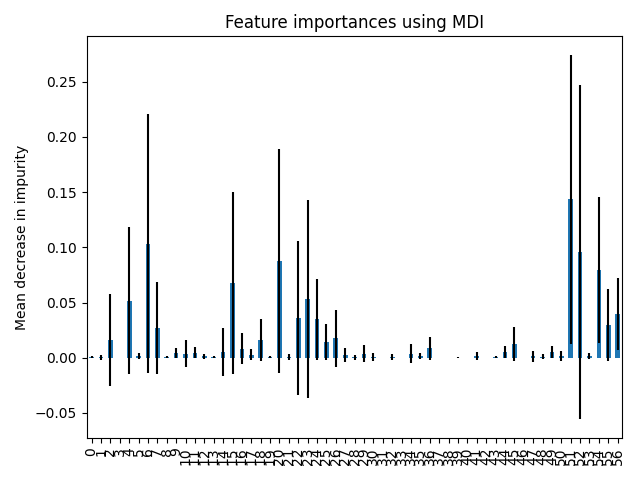
\includegraphics[width=0.7\linewidth]{../rfc_features}
					\caption{Features which reduce the standard deviation the most by adding them}
					\label{fig:rfcfeatures}
				\end{figure}
				In Fig. \ref{fig:rfcfeatures}, we see that the features at the beginning and end tend to be the most important as they have the highest values.
				
			\end{solution}
			\item {\bf Code:} Write a Python function {\tt eval\_gbdt(trainx, trainy, testx, testy, num\_estimators, learning\_rate)} that fits
			a GradientBoostingClassifier model to the training data. You can use {\tt sklearn} module for this part. The function should accept as input numpy 2d arrays, and return a dictionary containing the accuracy and AUC for the training and test sets and the predicted probabilities for the test set: {\tt return \{"train-acc": train\_acc, "train-auc": train\_auc, "test-acc": test\_acc, "test-auc": test\_auc, "test-prob": test\_prob\}}. The values for accuracy and AUC should be scalar numeric values, while test-prob should be a numpy 1-d array with the predicted probability for the positive class 1, for the test. Same format as HW2.
			\begin{solution}
				 Implimented in \texttt{q3.py}.
			\end{solution}
			\item {\bf Written:} Tune GBDT for the Spam classification problem by optimizing the hyperparameters {\tt num\_estimators} and {\tt learning\_rate} at least (you may choose to tune others). Use cross validation over the training set only. Report the best configuration, and the average AUC, F1, and Accuracy across validation folds.
			\begin{solution}
				We were able to iterate through many different estimators (1-15) and many different learning rates (0.1,0.01,0.001,0.0001,0.00001). We found the best was 12 estimatros and 0.0001 learing rate. The following was the results
				{'train-acc': 0.94932, 'train-auc': 0.94193, 'test-acc': 0.9275, 'test-auc': 0.91858, 'f1-score': 0.90794, 'test-prob': array([0.99657635, 0.00342365])}. This was better than NB on the last homework.
			\end{solution}
			\item {\bf Written:} Train GBDT on all training data with your best hyperparameters, and report AUC, F1, and Accuracy
			on the test set. Compare in a table to the performance of RF and NB. Comment on relative improvements / performance for this problem by the three different models.
			\begin{solution}
			Best Params:
			{'train-acc': 0.6153333333333333, 'train-auc': 0.5, 'test-acc': 0.5883822610868208, 'test-auc': 0.5, 'f1-score': 0.0, 'test-prob': array([0.61536766, 0.38463234])}
			This is much worse than NB. I don't know what happened but by training on the whole data set all at once, it didn't seem to work well.
			\end{solution}
		\end{enumerate}
		
	\end{enumerate}
	
	
	
	
	\section*{Acknowledgements}
	I would like to acknowledge that I attended both TA Swati's and TA Ziyang's office hours over the past week.
	
\end{document}
